\documentclass[onecolumn, draftclsnofoot,10pt, compsoc]{IEEEtran}
\usepackage{graphicx}
\usepackage{url}
\usepackage{caption}
\usepackage{setspace}
\usepackage{pdfpages}
\usepackage{geometry}
\geometry{textheight=9.5in, textwidth=7in}

\usepackage[]{parskip}
\usepackage{float}
\usepackage{listings}
\usepackage{xcolor}
\usepackage{pythonhighlight}

\def \CapstoneTeamName{		    Team 16}
\def \CapstoneTeamNumber{		16}
\def \GroupMemberOne{			Ian Brown}
\def \GroupMemberTwo{			Sean Gillen}
\def \GroupMemberThree{			Yihong Liu}
\def \CapstoneProjectName{		Radiation Spectrum Analysis Using Machine Learning}
\def \CapstoneSponsorCompany{	Oregon State University}
\def \CapstoneSponsorPerson{	Dr. Steve Reese}

\def \DocType{	%Problem Statement
				%Requirements Document
				%Technology Review
				%Design Document
				Progress Report
				}
			
\newcommand{\NameSigPair}[1]{\par
\makebox[2.75in][r]{#1} \hfil 	\makebox[3.25in]{\makebox[2.25in]{\hrulefill} \hfill		\makebox[.75in]{\hrulefill}}
\par\vspace{-12pt} \textit{\tiny\noindent
\makebox[2.75in]{} \hfil		\makebox[3.25in]{\makebox[2.25in][r]{Signature} \hfill	\makebox[.75in][r]{Date}}}}
% 3. If the document is not to be signed, un-comment the RENEW command below
\renewcommand{\NameSigPair}[1]{#1}

%%%%%%%%%%%%%%%%%%%%%%%%%%%%%%%%%%%%%%%
\begin{document}
\begin{titlepage}
    \pagenumbering{gobble}
    \begin{singlespace}
        \hfill 
        \par\vspace{.2in}
        \centering
        \scshape{
            \huge CS Capstone \DocType \par
            {\large\today}\par
            \vspace{.5in}
            \textbf{\Huge\CapstoneProjectName}\par
            \vfill
            {\large Prepared for}\par
            \Huge \CapstoneSponsorCompany \par
            \vspace{5pt}
            {\Large\NameSigPair{\CapstoneSponsorPerson}\par}
            {\large Prepared by }\par
            Radiological Counting\par
            \vspace{5pt}
            {\Large
                \NameSigPair{\GroupMemberOne}\par
                \NameSigPair{\GroupMemberTwo}\par
                \NameSigPair{\GroupMemberThree}\par
            }
            \vspace{20pt}
        }
        \begin{abstract}
        The capstone team has finished the beta version of a system to identify the radioactive isotopes present in a sample using real-time data from a gamma-ray spectrometer.
        The goal is to get the result more quickly than from the conventional methods used in software such as Ortec GammaVision.
        The system uses machine learning classifiers to return confidence values for the presence of each isotope in its training set, and returns a result when a threshold confidence value of 0.9999 is reached.
        To explore their respective abilities in this domain, three different types of classifier are used simultaneously: naive Bayes, neural network, and decision tree.
        Currently, the naive Bayes model is working well but the other two models are too slow.
        The team is working to improve this, but the project's main goal of quick radioisotope identification has been achieved.
        \end{abstract}
    \end{singlespace}
\end{titlepage}
\newpage
\pagenumbering{arabic}
\tableofcontents
% 7. uncomment this (if applicable). Consider adding a page break.
%\listoffigures
%\listoftables
\clearpage

\section{Project Recap}
The group will demonstrate a proof-of-concept reduction in spectroscopy classification time through the use of machine learning, following an algorithm developed collaboratively at OSU and Georgetown University.
To do so, the team will use radiation counting data collected by an analogous detector set up at the Oregon State University Training, Research, Isotopes, General Atomics (TRIGA) reactor.
Three different machine learning models will be trained and tested with this data to identify the radioisotopes present with shorter time and higher accuracy than the current technology, such as Ortec GammaVision, Listmode.

\section{Current Progress}
Currently, our client considers our project to be just about done.
We have implemented all three of the classifiers requested in the project proposal.
Additionally, we are able to parse the spectrum file in real time and run one of our classifiers repeatedly as new data is written by the detector.
The client has told us that the only main thing left for us to do is to compare the performance of our application to the GammaVision software used by him.
Aside from this, we will also work on polishing and performance optimization.

\section{Remaining Work}

\subsection{Neural Network}
What we have left to do for neural network machine learning model is to reduce the run time of classifying different source isotope and optimize the algorithm if possible. For now, the neural network has a consistent and high accuracy of classifying different isotopes, but it takes much longer to classify than other models, especially for the mixed sample, such as a sample contain the cs, co, ba. what we can do is to implement a package from scikit-learn called GrindSearchCV to find the best value for each parameter and implement it see if the running time can be reduced. 

\subsection{Naive Bayes}
The Naive Bayes classifier currently seems to be performing the best of all three.
After discussing this with the client, we agreed that our next step will be to compare the performance of this model to the GammaVision software.
This software is used by the client to do normal isotope identification.
If our model is able to outperform it, the client will consider the project successful.

We plan to do this test by first taking various samples of a material for different time intervals.
Then, we will use GammaVision on each of these samples to find the minimum time interval that the software is able to correctly identify the isotopes.
We will then run our model on a real-time sample of the material.
Once the model has made a correct prediction, we will compare the time it took to the minimum time interval required by GammaVision.
Based on our previous tests with our model, we believe that our model will be able to pass this test.

\subsection{Decision Tree}
The decision tree classifier is currently the least accurate of the three, so the main work will be in improving this classifier's accuracy. 
It does much better than random chance, but sometimes identifies Co-60 and Ba-133 when they are not present in the sample.

\section{Problems}
While the team was able to implement all three types of classifiers, the performance varies between each of them.
In particular, the naive Bayes classifier appears to perform the best so far, while the neural network and decision tree models are taking too long in their predictions.
The neural network classifier is likely slow because it is fairly more complex than most models.
However, this may also be due to the fact that we don't have enough data available.
The decision tree model is slow because, in order to have a good probability metric, multiple decision trees are needed.
Adding more trees improves the accuracy of the predictions at the cost of speed.
While there may not be much we can do to solve these issues, we will continue to experiment with both of these models.

\section{Code}
\subsection{Real time parsing code}
This code contains the logic for parsing the file created by the detector in real time.
The callable parameter \texttt{on\_adc} is invoked every time a new ADC event is parsed.

\begin{python}
def with_parser(file: BinaryIO, on_adc: Callable[[int], bool]) -> None:
    """
    Parse an Ortec binary file and execute closure for each ADC event
    encountered
    :param file BinaryIO: Binary file
    :param on_adc Callable[[int], bool]: Closure executed for each ADC event.
    If the returned value is truthy, parsing will stop.
    """
    while True:
        raw_word = file.read(WORD_SIZE_BYTES)
        if not raw_word:
            return
        # read word in as little-endian 32-bit unsigned int
        word = struct.unpack("<I", raw_word)[0]

        # don't need mask because it's the 2 MSB
        prefix = word >> PREFIX_BIT_SHIFT

        # ignoring words with time and other data for now
        if prefix == PREFIX_ADC:
            # need mask to remove prefix bits after shift
            channel = (word >> CHANNEL_BIT_SHIFT) & CHANNEL_MASK
            if on_adc(channel):
                return
\end{python}

\subsection{Machine learning model creation and real time test code}
This code shows how our machine learning models are created, trained, evaluated, and tested on the data set.
This example shows the code for the Naive Bayes model, but the structure looks mostly the same for the other two classifiers as well.

\begin{python}
from functools import partial
import timeit
from typing import List

import numpy as np
from sklearn.model_selection import cross_val_score
from sklearn.multioutput import MultiOutputClassifier
from sklearn.naive_bayes import MultinomialNB
from sklearn.preprocessing import MultiLabelBinarizer

from ortec_file_utils import get_training_data
from serializer import Serializer


def bin_list(arr: List[int], bin_size: int):
    sp = np.array_split(arr, bin_size)
    sums = [part.sum() for part in sp]
    return sums


labels: List[str] = ['Cs-137', 'Ba-133', 'Co-60']
mlb = MultiLabelBinarizer()
mlb.fit([labels])


def print_proba(results: List[List[int]]):
    print('Probabilities:\n\t' + '\n\t'.join([
        f'{mlb.classes_[idx]}:\t{prob[0]}' for idx, prob in enumerate(results)
    ]))


def print_prediction(results: List[List[int]]):
    print(f'Prediction: {mlb.inverse_transform(results)[0]}')


num_training_lists = 10
print(f'Using {num_training_lists} snapshots from each spectrum')

bin_size = 10
# print(f'Using {bin_size} bins')
bin_train = partial(bin_list, bin_size=bin_size)

sample_files = {
    'cs.dat': {'labels': ['Cs-137']},
    'ba.dat': {'labels': ['Ba-133']},
    'co.dat': {'labels': ['Co-60']},
    '2020-01-31_co_ba.dat': {'labels': ['Ba-133', 'Co-60']},
    '2020-01-31_cs_ba.dat': {'labels': ['Ba-133', 'Cs-137']},
    '2020-01-31_cs_co.dat': {'labels': ['Co-60', 'Cs-137']},
    'ba_co_cs.dat': {'labels': ['Ba-133', 'Co-60', 'Cs-137']}
}

for key, value in sample_files.items():
    value['data'] = get_training_data("data/" + key, num_training_lists)

# Combine all the training data arrays into one big feature set
X = np.vstack(list(map(lambda x: x['data'], sample_files.values())))
# X = normalize(X)

# Build a label list that corresponds to the feature set
y = []
for value in sample_files.values():
    y += [value['labels']]*len(value['data'])
y = np.array(mlb.transform(y))

# Use a multi-label classifier implementing Multinomial Naive Bayes
clf = MultiOutputClassifier(MultinomialNB())
clf.fit(X, y)

print(f'Mean accuracy: {clf.score(X, y)}')

num_folds = 10
cv_score = cross_val_score(clf, X, y, cv=num_folds)
print(f'{num_folds}-fold cross-validation: {cv_score}')

# Perform real-time tests for each input file
for key, value in sample_files.items():
    print("\nPerforming real-time classification of "
          f"{', '.join(value['labels'])}")
    start_time = timeit.default_timer()
    features = Serializer("data/" + key).classify_realtime(clf)
    total_time = timeit.default_timer() - start_time
    print(f'Classified in {total_time} seconds')
    print_prediction(clf.predict(features))
    print_proba(clf.predict_proba(features))
\end{python}

\section{Project Images}
\subsection{Neural Network Demo Result}
\begin{figure}[H]
    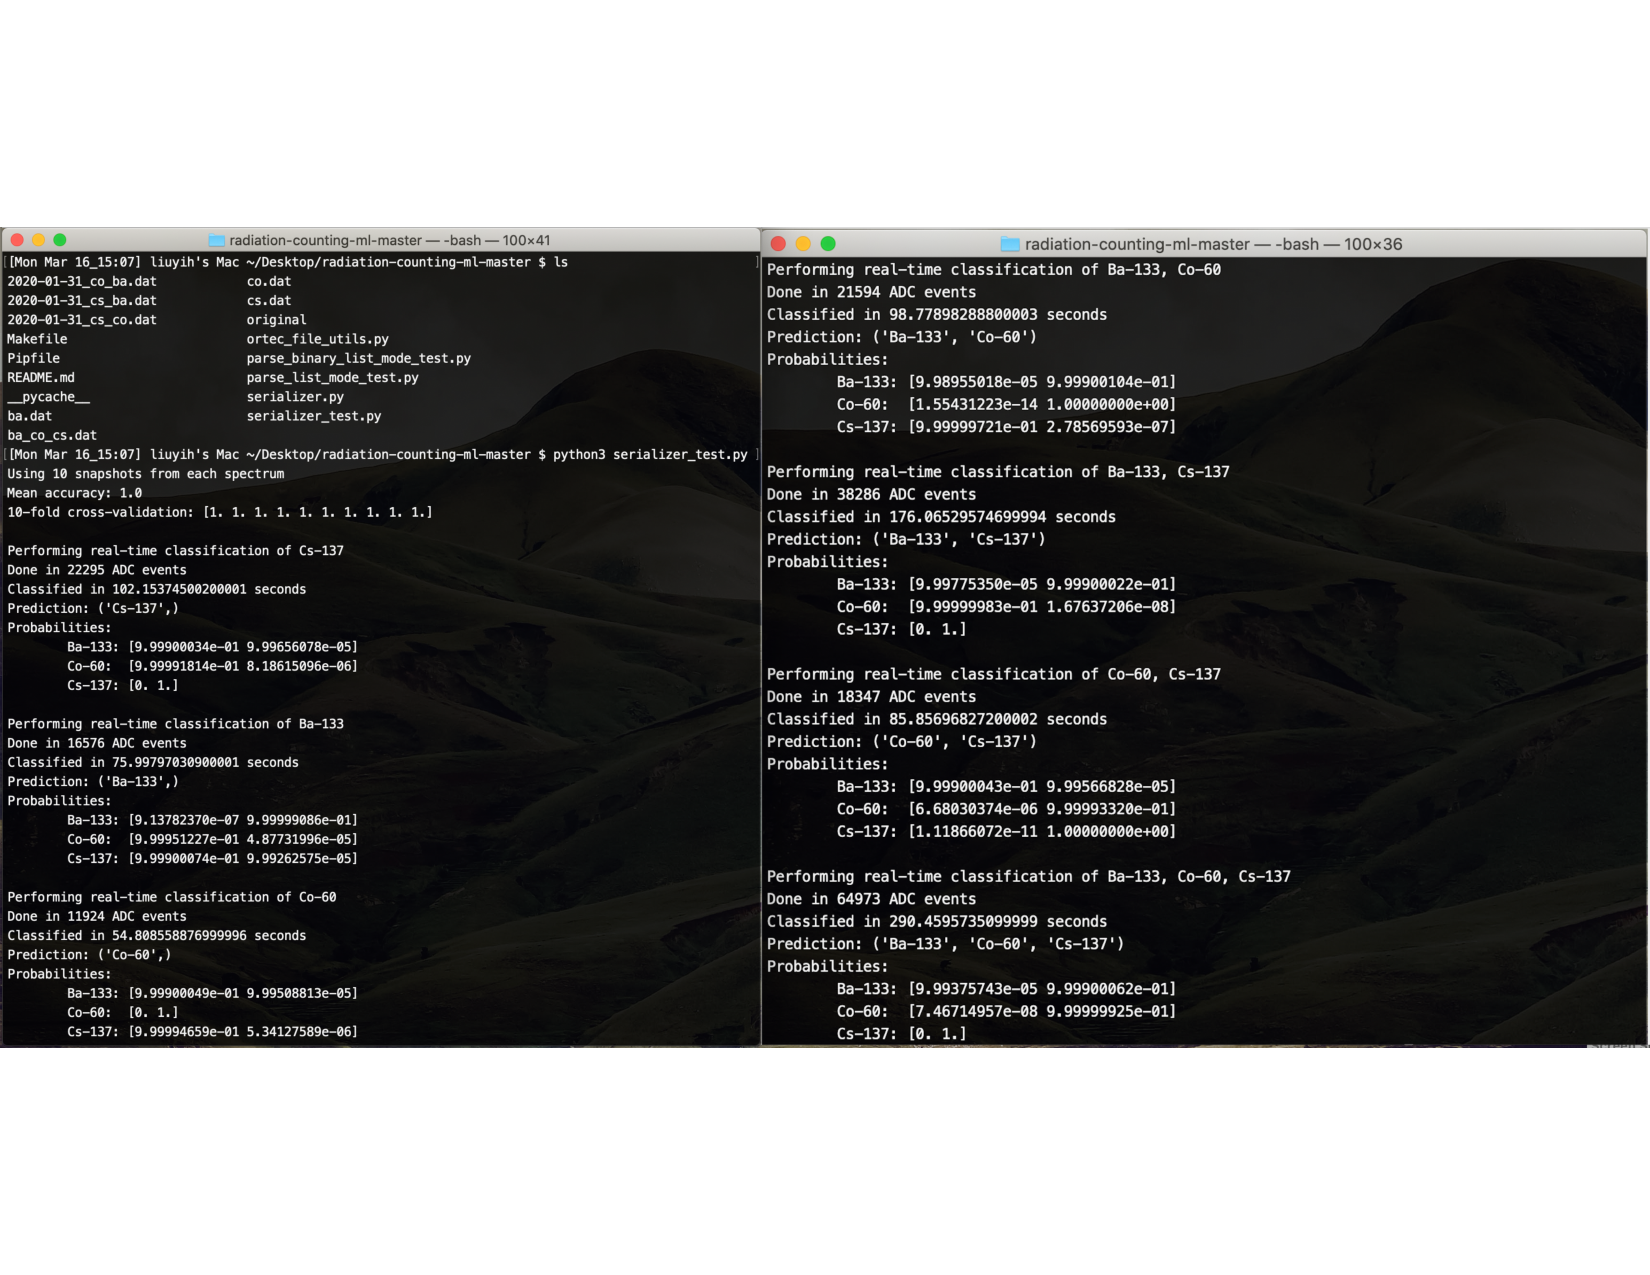
\includegraphics[width=\linewidth]{neural_network demo screenshot.pdf}
\end{figure}

\subsection{Naive Bayes Demo Result}
\begin{figure}[H]
    \includegraphics[width=\linewidth]{naive-bayes-demo-split.png}
\end{figure}

\subsection{Decision Tree Demo Result}
\begin{figure}[H]
    \includegraphics[width=\linewidth]{decision-tree-demo-split.png}
\end{figure}

\end{document}